\documentclass{standalone}
\usepackage{tikz}
\usepackage{ctex,siunitx}
\setCJKmainfont{Noto Serif CJK SC}
\usepackage{tkz-euclide}
\usepackage{amsmath}
\usepackage{wasysym}
\usetikzlibrary{patterns, calc}
\usetikzlibrary {decorations.pathmorphing, decorations.pathreplacing, decorations.shapes,}
\begin{document}
\small
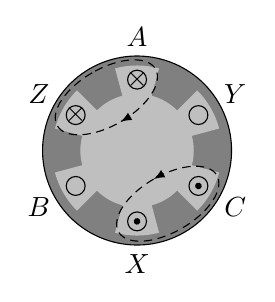
\begin{tikzpicture}[>=latex,scale=1.2]
  % \useasboundingbox(0.9,0)rectangle(5.1,5);
  \begin{scope}[rotate=120]
  \draw[fill=gray](0,0)circle(1);
  \fill[lightgray](0:0.6)arc(0:15:0.6)--(15:0.9)arc(15:45:0.9)--(45:0.6)arc(45:60:0.6)
  \foreach \x in {60,120,180,240,300}
  { arc(\x:\x+15:0.6)--(\x+15:0.9)arc(\x+15:\x+45:0.9)--(\x+45:0.6)arc(\x+45:\x+60:0.6) };
  \draw[densely dashed,postaction={decorate},decoration={markings,mark=at position 0.5 with {\arrowreversed{>}}}](0.65,0)ellipse(0.3 and 0.6);
  \draw[densely dashed,postaction={decorate},decoration={markings,mark=at position 0 with {\arrow{>}}}](-0.65,0)ellipse(0.3 and 0.6);
  \fill(150:0.75)circle(1pt)(210:0.75)circle(1pt);
  \node at (30:0.75){$\times$};
  \node at (-30:0.75){$\times$};
  \end{scope}
  \foreach \x/\y in {30/Y,90/A,150/Z,210/B,270/X,330/C}
  {
    \node at (\x:1.2) [inner sep=0pt]{$\y$};
    \draw(\x:0.75)circle(0.1);
  }
\end{tikzpicture}
\end{document}